\documentclass{my_pracamgr}

\usepackage{lmodern}
\usepackage{upgreek}
\usepackage[utf8]{inputenc}
\usepackage{graphicx}
\usepackage{listings}
\usepackage{epstopdf}
\usepackage{hyperref}
\usepackage{color}
\usepackage{listings}
\usepackage{textcomp}
\usepackage[polish,english]{babel}
\usepackage[T1]{fontenc}
\usepackage{subfig}
\usepackage{verbatim}
\usepackage{float}
\newcommand{\me}{\mathrm{e}}

\author{Elena Shylko}

\nralbumu{320957}

\title{Tight Binding method for electronic structure of two-dimensional nanostructures}

\tytulang{Metoda ciasnego wiązania dla struktury elektronowej nanostruktur dwuwymiarowych}

\kierunek{Mathematical and computer modeling of physical processes}

\opiekun{Prof. Jacek A. Majewski\\
  Chair of Condensed Matter Physics\\
  }

\date{June 2016}

\dziedzina{ 
13.2 Physics\\ 
}

\def\category#1#2#3{%
    \begingroup
        \let\and\relax
            #1 [\textbf{#2}]%
                \if!#3!\else : #3\fi
    \endgroup
}
\klasyfikacja{
\category{71.15.Ap}{Methods of electronic structure calculations}{Basis sets (LCAO, plane-wave, APW, etc.) and related methodology (scattering methods, ASA, linearized methods, etc.)} \\
\category{71.15.Dx}{Methods of electronic structure calculations}{Computational methodology (Brillouin zone sampling, iterative diagonalization, pseudopotential construction).} \\
\category{73.22.Pr}{Electronic structure of nanoscale materials and related systems}{Electronic structure of graphene.}  }

\keywords{Tight binding, modelling, electronic sructure, low-dimensional materials, graphene}


\begin{document}
\maketitle

\begin{abstract}
 Very brief story.
\end{abstract}

\tableofcontents
%\listoffigures
%\listoftables

\chapter{Introduction}
\label{ch:introduction}
Tight-binding (TB) method is an approach to the calculation of energy band structure of various materials, where electrons are tightly bound to the atom to which they belongs. So that an approximate set of wave functions based upon superposition of wave functions for isolated atoms located at atomic sites is used.

TB method was developed by F. Bloch \cite{bloch} in 1928.  Bloch considered only the $s$ atomic orbital. In 1934 H. Jones, N. F. Mott and H. W. B. Skinner \cite{mott} considered wave functions constructed by solving a secular problem between $s$, $p_x$, $p_y$ and $p_z$ Bloch functions.

Package code and example inputs are placed in open repository \url{https://github.com/Lenka42/TightBinding}.
\chapter{Tight Binding method}
\label{ch:theory}
\section{Introduction to the tight-binding model}
Tight-binding method is developed to describe band structure of various materials, where electrons are localized at the atomic positions (tight-bonded to the atoms). In TB model simple effective hamiltonian is used in contrast to first-principle calculations. 

The most essential approximation in TB model is the so-called two-center approximation, where Hamiltonian is approximated by the atomic Hamiltonian centered on the atomic positions in the unit cell $\vec{R}$ and only two-centered integrals are encountered.

We construct the Bloch wave function of the crystal as a linear combination of the local Wannier functions, which are approximated by the eigenfunctions of the atomic Hamiltonian, the atomic orbitals $\phi_{\nu, s}(\vec{r} - \vec{t_i} - \vec{R})$, where $\vec{t_j}$ is the position of atom $i$ in the unit cell at $\vec{R}$ and $s$ is the spin of $\nu$th orbital. The Bloch wave function
\begin{equation} \label{eq:wave_fun}
\Psi_{\vec{k}, j ,\nu, s} = \frac{1}{\sqrt{N}} \sum_{\vec{R}} \me^{i\vec{k}\vec{R}} \phi_{\nu, s} (\vec{r} - \vec{t_j} - \vec{R})
\end{equation}
satisfies Bloch theorem.

Starting with Schr\"{o}dinger equation,
\begin{equation}
\hat{H}\Psi_{\vec{k}}(\vec{r}) = \epsilon_{\vec{k}} \Psi_{\vec{k}}(\vec{r})
\end{equation}
and expanding crystal wave function in the basis of the on-site Bloch wave functions
\begin{equation}
\Psi_{\vec{k}}(\vec{r}) = \sum_j c_{\vec{k}, j} \Psi_{\vec{k}, j}(\vec{r})
\end{equation}
basing on variational principle one can derive the secular equation,
\begin{equation} \label{eq:secular}
\sum_j[H_{i,j}(\vec{k}) - \epsilon_{\vec{k}} S_{i, j}(\vec{k})] c_{\vec{k}, j} = 0.
\end{equation}
Where two-center Hamiltonian and overlap matrix elements are defined by the integrals:
\begin{equation} \label{eq:h_matrix}
H_{i,j}(\vec{k}) = \frac{1}{N} \sum_{\vec{R}, \vec{R'}} \int d \vec{r} \phi_i^*(\vec{r} - \vec{R'}) \hat{H}(\vec{r} - \vec{R}) \phi_j(\vec{r} - \vec{R}),
\end{equation}
\begin{equation} \label{eq:s_matrix}
S_{i,j}(\vec{k}) = \frac{1}{N} \sum_{\vec{R}, \vec{R'}} \int d \vec{r} \phi_i^*(\vec{r} - \vec{R'}) \phi_j(\vec{r} - \vec{R}).
\end{equation}

Usually integration results are taken as parameters, which have to be fitted to reproduce certain solid's properties or the band structure calculated by first-principle approach. Matrix Elements in \ref{eq:h_matrix} and \ref{eq:s_matrix} where $\vec{R} = \vec{R'}$ are called on-site elements, and for $\vec{R} \neq \vec{R'}$ they are called hopping and overlap parameters respectively. 

In general case, atomic orbitals centered on different sites are not orthogonal and the corresponding overlap parameters have small but finite values.But often orthogonal basis of orbitals is used, so that overlap matrix becomes identity matrix and energies are eigenvalues of the Hamiltonian matrix. In the following sections I will discuss both approaches. 

The next approximation is to consider a finite as small as necessary number of orbitals per atom. The number of solutions of the secular equation in \ref{eq:secular} is equal to dimension of the Hamiltonian matrix,
\begin{equation}
dim = g \times \sum_j n_j
\end{equation}
Here $g$ is spin factor ($1$ or $2$), summation goes through all atoms in unit cell and $n_j$ is number of included orbitals for atom $j$.

In the final nearest neighbors approximation (NNA) only the nearest neighbors of a chosen atom are taken into account in the Hamiltonian and overlap matrix elements Eqs. (\ref{eq:h_matrix}) and (\ref{eq:s_matrix}).
\section{Spin-orbit interaction }


\chapter{Current results}\label{r:results}
\section{Diamond}
I investigated diamond crystal. I considered here the case where we have only one set of $s$, $p_z$, $p_y$, and $p_z$ orbitals at each
atomic site.
\begin{figure}[h] 
 \begin{center}
  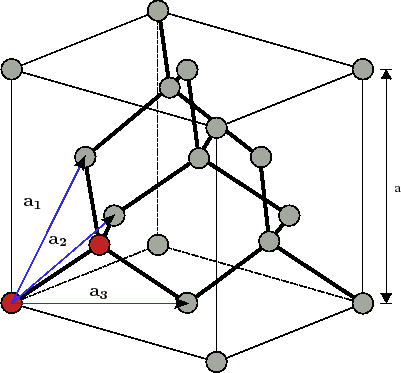
\includegraphics[width=0.3\linewidth]{img/diamond_crystall}
  \caption{Diamond crystall structure.}
 \end{center}
\end{figure}

\begin{table}[h]
 \begin{center}
  \begin{tabular}{|c|c|}
  \hline
    Parameter&Value, [eV]\\ \hline
    $\epsilon_s$ & $0.0$ \\ \hline
    $\epsilon_p$ & $7.4$ \\ \hline
    $V_{\sigma ss}$ & $-3.8$  \\ \hline
    $V_{\sigma sp}$ & $4.44$\\ \hline
    $V_{\sigma pp}$ & $-1.325$ \\ \hline
    $V_{\pi pp}$ &  $4.9$\\ \hline
  \end{tabular}
 \end{center}
  \caption{Interaction parameters for diamond.}
\end{table}

\begin{figure} 
  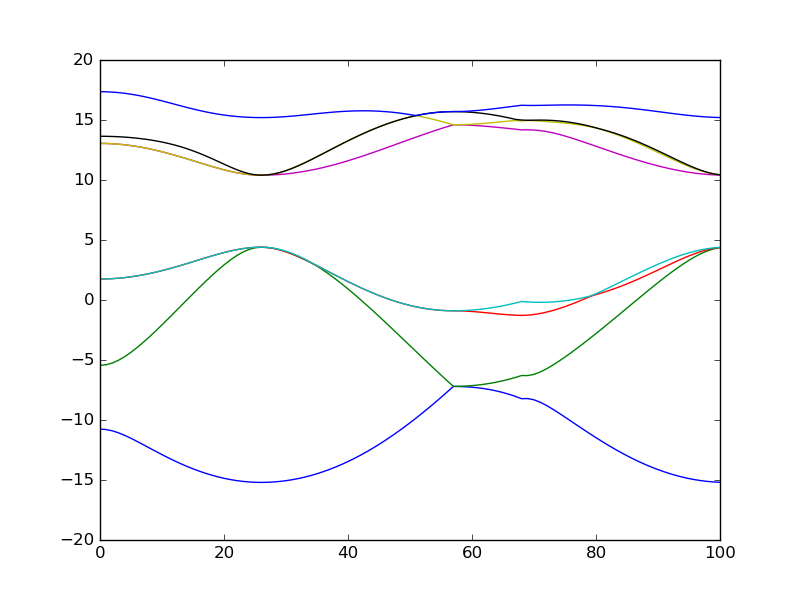
\includegraphics[width=\linewidth]{img/diamond_sp}
  \caption{Calculated band structure of diamond.}
\end{figure}
\begin{figure} 
\begin{center}
  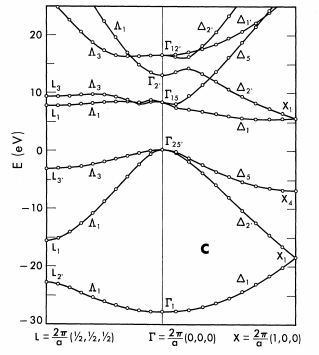
\includegraphics[width=0.5\linewidth]{img/diamond_exp_band_struct}
  \caption{Band structure of diamond (experiment).}
\end{center}
\end{figure}  

\newpage
\section{Molybdenum disulfide (monolayer)}
In my TB model I adopted a non-orthogonal basis set of $sp_3 d_5$ orbitals considering only the nearest neighbour interactions between following pairs of atoms: $Mo - S$, $Mo-Mo$, $S-S$.
\begin{minipage}{\linewidth}
\begin{verbatim}
{0: [(1, array([ 0.        ,  1.80133284,  1.555     ])), 
     (2, array([ 0.        ,  1.80133284, -1.555     ])), 
     (0, array([-1.56      , -2.70199926,  0.        ])), 
     (1, array([-1.56      , -0.90066642,  1.555     ])), 
     (2, array([-1.56      , -0.90066642, -1.555     ])), 
     (0, array([-3.12,  0.  ,  0.  ])), 
     (0, array([ 1.56      , -2.70199926,  0.        ])), 
     (1, array([ 1.56      , -0.90066642,  1.555     ])), 
     (2, array([ 1.56      , -0.90066642, -1.555     ])), 
     (0, array([-1.56      ,  2.70199926,  0.        ])), 
     (0, array([ 3.12,  0.  ,  0.  ])), 
     (0, array([ 1.56      ,  2.70199926,  0.        ]))], 
 1: [(0, array([ 0.        , -1.80133284, -1.555     ])), 
     (2, array([ 0.  ,  0.  , -3.11])), 
     (1, array([-1.56      , -2.70199926,  0.        ])), 
     (1, array([-3.12,  0.  ,  0.  ])), 
     (1, array([ 1.56      , -2.70199926,  0.        ])), 
     (0, array([-1.56      ,  0.90066642, -1.555     ])), 
     (1, array([-1.56      ,  2.70199926,  0.        ])), 
     (1, array([  3.12000000e+00,  -4.44089210e-16,   0.00000000e+00])), 
     (0, array([ 1.56      ,  0.90066642, -1.555     ])), 
     (1, array([ 1.56      ,  2.70199926,  0.        ]))],
 2: [(0, array([ 0.        , -1.80133284,  1.555     ])), 
     (1, array([ 0.  ,  0.  ,  3.11])), 
     (2, array([-1.56      , -2.70199926,  0.        ])), 
     (2, array([-3.12,  0.  ,  0.  ])), 
     (2, array([ 1.56      , -2.70199926,  0.        ])), 
     (0, array([-1.56      ,  0.90066642,  1.555     ])), 
     (2, array([-1.56      ,  2.70199926,  0.        ])), 
     (2, array([  3.12000000e+00,  -4.44089210e-16,   0.00000000e+00])), 
     (0, array([ 1.56      ,  0.90066642,  1.555     ])), 
     (2, array([ 1.56      ,  2.70199926,  0.        ]))]})
\end{verbatim}
\end{minipage}
\begin{figure} 
\begin{center}
  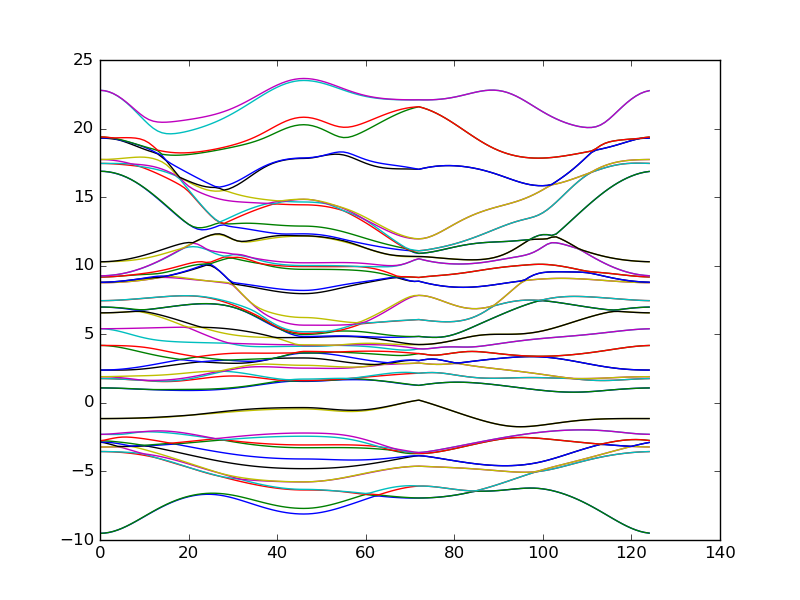
\includegraphics[width=\linewidth]{img/mos2_mono_soc_S}
  \caption{Calculated band structure of $MoS_2$.}
\end{center}
\end{figure}  
\begin{figure} 
\begin{center}
  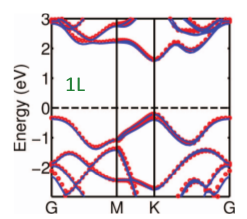
\includegraphics[width=0.5\linewidth]{img/MoS2_lit_band_struc}
  \caption{Band structure of $MoS_2$ (literature)).}
\end{center}
\end{figure}  

\newpage
\section{Graphene}
\begin{figure}[h] 
\begin{center}
  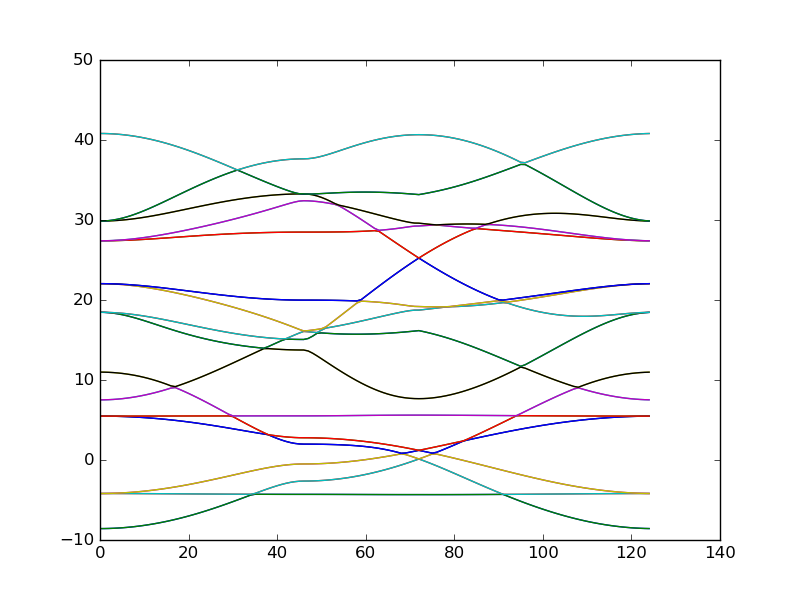
\includegraphics[width=0.55\linewidth]{img/graphene_pd_soc}
  \caption{Calculated Band structure of graphene ($p_3d_5$)).}
\end{center}
\end{figure}
\begin{figure}[h] 
\begin{center}
  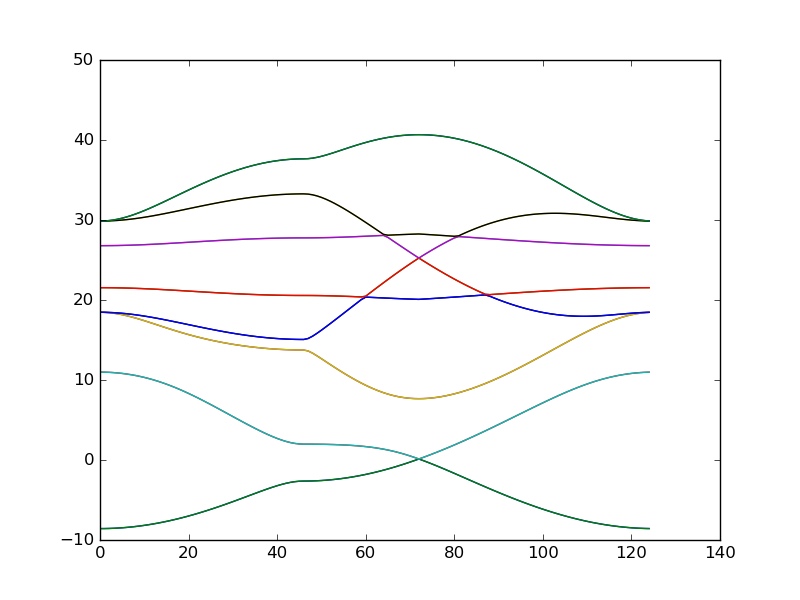
\includegraphics[width=0.55\linewidth]{img/graphene_pd_soc3}
  \caption{Calculated Band structure of graphene ($p_zd_{xz}d_{yz}$)).}
\end{center}
\end{figure}

\chapter{Podsumowanie}

\begin{itemize}
\item realizacja zimnej reakcji lambliarnej,
\item loty celulityczne,
\item dokadne obliczenie wieku Wszechswiata.
\end{itemize}

\section{Perspektywy wykorzystania w przemysle}

Ze wzgledu na znaczenie strategiczne wynikow pracy ten punkt ulegl
utajnieniu.

\appendix

\chapter{Glowna petla programu zapisana w jezyku T\=oFoo}

\begin{verbatim}
[[foo]{,}[[a3,(([(,),{[[]]}]),
  [1; [{,13},[[[11],11],231]]].
  [13;[!xz]].
  [42;[{,x},[[2],{'a'},14]]].
  [br;[XQ*10]].
 ), 2q, for, [1,]2, [..].[7]{x}],[(((,[[1{{123,},},;.112]],
        else 42;
   . 'b'.. '9', [[13141],{13414}], 11),
 [1; [[134,sigma],22]].
 [2; [[rho,-],11]].
 )[14].
 ), {1234}],]. [map [cc], 1, 22]. [rho x 1]. {22; [22]},
       dd.
 [11; sigma].
        ss.4.c.q.42.b.ll.ls.chmod.aux.rm.foo;
 [112.34; rho];
        001110101010101010101010101010101111101001@
 [22%f4].
 cq. rep. else 7;
 ]. hlt
\end{verbatim}

\chapter{Przykladowe dane wejsciowe algorytmu}

\begin{center}
  \begin{tabular}{rrr}
    $\alpha$ & $\beta$ & $\gamma_7$ \\
    901384 & 13784 & 1341\\
    68746546 & 13498& 09165\\
    918324719& 1789 & 1310 \\
    9089 & 91032874& 1873 \\
    1 & 9187 & 19032874193 \\
    90143 & 01938 & 0193284 \\
    309132 & $-1349$ & $-149089088$ \\
    0202122 & 1234132 & 918324098 \\
    11234 & $-109234$ & 1934 \\
  \end{tabular}
\end{center}

\chapter{Przykladowe wyniki blabalizy
    (ze wspolczynnikami~$\sigma$-$\rho$)}

\begin{center}
  \begin{tabular}{lrrrr}
    & Wspolczynniki \\
    & Gombaskiego & $\rho$ & $\sigma$ & $\sigma$-$\rho$\\
    $\gamma_{0}$ & 1,331 & 2,01 & 13,42 & 0,01 \\
    $\gamma_{1}$ & 1,331 & 113,01 & 13,42 & 0,01 \\
    $\gamma_{2}$ & 1,332 & 0,01 & 13,42 & 0,01 \\
    $\gamma_{3}$ & 1,331 & 51,01 & 13,42 & 0,01 \\
    $\gamma_{4}$ & 1,332 & 3165,01 & 13,42 & 0,01 \\
    $\gamma_{5}$ & 1,331 & 1,01 & 13,42 & 0,01 \\
    $\gamma_{6}$ & 1,330 & 0,01 & 13,42 & 0,01 \\
    $\gamma_{7}$ & 1,331 & 16435,01 & 13,42 & 0,01 \\
    $\gamma_{8}$ & 1,332 & 865336,01 & 13,42 & 0,01 \\
    $\gamma_{9}$ & 1,331 & 34,01 & 13,42 & 0,01 \\
    $\gamma_{10}$ & 1,332 & 7891432,01 & 13,42 & 0,01 \\
    $\gamma_{11}$ & 1,331 & 8913,01 & 13,42 & 0,01 \\
    $\gamma_{12}$ & 1,331 & 13,01 & 13,42 & 0,01 \\
    $\gamma_{13}$ & 1,334 & 789,01 & 13,42 & 0,01 \\
    $\gamma_{14}$ & 1,331 & 4897453,01 & 13,42 & 0,01 \\
    $\gamma_{15}$ & 1,329 & 783591,01 & 13,42 & 0,01 \\
  \end{tabular}
\end{center}

\begin{thebibliography}{99}
\addcontentsline{toc}{chapter}{Bibliography}

\bibitem{bloch} F. Bloch, \textit{Über die Quantenmechanik der Elektronen in Kristallgittern}, Z. Phys. (1928), vol. 52: 555–600
\bibitem{mott} H. Jones, N. F. Mott,  H. W. B. Skinner, \textit{A Theory of the Form of the X-Ray Emission Bands of Metals}, Phys. Rev. 45, 379 (1934)
\bibitem{slatter} J. C. Slater, G. F. Koster, \textit{Simplified LCAO Method for the Periodic Potential Problem}, Phys. Rev. 94, 1498 (1954)
\bibitem{kittel} C. Kittel, \textit{Introduction to Solid State Physics, 7th ed.}, Wiley, (1996) 
\bibitem{soc} R. J. Elliott, \textit{Theory of the effect of spin-orbit coupling on magnetic reso-
nance in some semiconductors}, Phys. Rev. 96(2):266–279 (1954).
\bibitem{temperature} A. Radkowsky, \textit{Temperature Dependence of Electron Energy Levels in Solids}, Phys. Rev. 73, 749 (1948)
\bibitem{diamond} W. Saslow, T. K. Bergstresser, Marvin I. Cohen, \textit{Band structure and optical properties of diamond}, Phys. Rev. 16, 9 (1966)
\bibitem{mos2} K. F. Mak, C. Lee, J. Hone, J. Shan, T. F. Heinz, \textit{Atomically Thin $MoS_2$: A New Direct-Gap Semiconductor}, Phys. Rev. Lett. 105, 136805 (2010)
\bibitem{geim} Andre K. Geim, \textit{Nobel Lecture: Random walk to graphene}, Rev. Mod. Phys. 83, 851 (2011)
\bibitem{brodie} B.C. Brodie, \textit{On the Atomic Weight of Graphite},  Philosophical Transactions of the Royal Society of London 149: 249–259 (1859)
\bibitem{debije} P. Debije, P. Scherrer. \textit{Interferenz an regellos orientierten Teilchen im Röntgenlicht I}, Physikalische Zeitschrift (in German) 17: 277 (1916)
\bibitem{bernal} J. D. Bernal, \textit{The Structure of Graphite}, Proc. R. Soc. Lond. A106 (740): 749–773 (1924)
\bibitem{haenni} V. Kohlschütter, P. Haenni, \textit{Zur Kenntnis des Graphitischen Kohlenstoffs und der Graphitsäure}, Zeitschrift für anorganische und allgemeine Chemie (in German) 105 (1): 121–144  (1919)
\bibitem{wallace} P. R. Wallace, \textit{The Band Structure of Graphite}, Physical Review 71: 622–634 (1947)
\bibitem{divincenzo} D. P. DiVincenzo, E. J. Mele, \textit{Self-Consistent Effective Mass Theory for Intralayer Screening in Graphite Intercalation Compounds}, Physical Review B 295 (4): 1685–1694 (1984)
\bibitem{epitaxial} C. Oshima, A. Nagashima, \textit{Ultra-thin epitaxial films of graphite and hexagonal boron nitride on solid surfaces}, J. Phys.: Condens. Matter 9: 1–20. (1997)
\bibitem{geim-science} K. S. Novoselov, A. K. Geim, S. V. Morozov, D. Jiang; Y. Zhang, S. V. Dubonos, I. V. Grigorieva, A. A. Firsov, \textit{Electric Field Effect in Atomically Thin Carbon Films}, Science 306 (5696): 666–669 (2004)
\bibitem{graphene_review} A. H. Castro Neto et al., \textit{The electronic properties of graphene}, Rev. Mod. Phys., Vol. 81, No. 1, January–March (2009)
\bibitem{boukhvalov} D. W. Boukhvalov, M. I. Katsnelson, A. I. Lichtenstein, \textit{Hydrogen on graphene: Electronic structure, total energy, structural distortions and magnetism
from first-principles calculations}, Phys. Rev. B 77, 035427 (2008)
\bibitem{basics} B. Gharekhanlou, S. Khorasani, \textit{An overview of tight-binding method for two-dimensional carbon structures}, Graphene: synthesis and applications (2011)
\bibitem{slonczewski} J. C. Slonczewski, P. R. Weiss, \textit{Band Structure of Graphite}, Phys. Rev. 109, 272 (1958)
\bibitem{graphene_soc_parameters} T. B. Boykin, M. Luisier, G. Klimeck, X. Jiang, N. Kharche, Y. Zhou, S. K. Nayak, \textit{Accurate six-band nearest-neighbor tight-binding model for the $\pi$-bands of bulk graphene and graphene nanoribbons}, J. Appl. Phys. 109, 104304 (2011)
\bibitem{brei} L. Brey, H. A. Fertig, \textit{Electronic states of graphene nanoribbons studied with the Dirac equation}, Phys. Rev. B 73, 235411 – Published 15 June (2006)
\bibitem{areshkin} D. A. Areshkin, D. Gunlycke, C. T. White, \textit{Ballistic transport in graphene nanostrips in the presence of disorder: importance of edge effects}, Nano Lett. 7, 204 (2007)
\bibitem{barone} V. Barone, O. Hod, G. E. Scuseria, \textit{Electronic structure and stability of semiconducting graphene nanoribbons}, Nano Lett. 6, 2748 (2006)
\bibitem{han} M. Y. Han., B. Özyilmaz, Y. Zhang, P. Kim,\textit{Energy Band-Gap Engineering of Graphene Nanoribbons}, Physical Review Letters 98 (20): 206805 (2007)
\end{thebibliography}


\end{document}


%%% Local Variables:
%%% mode: latex
%%% TeX-master: t
%%% coding: latin-2
%%% End:
